\documentclass[11pt]{article}

\usepackage[margin=1in]{geometry}
\usepackage{amsmath,amssymb}
\usepackage{graphicx}
\usepackage{booktabs}
\usepackage{hyperref}
\usepackage{xcolor}
\usepackage[numbers,sort&compress]{natbib}
\usepackage{caption}
\usepackage{listings}
\usepackage{enumitem}

\hypersetup{
  colorlinks=true,
  linkcolor=blue!50!black,
  citecolor=blue!50!black,
  urlcolor=blue!50!black
}

\newcommand{\code}[1]{\texttt{#1}}
% Plain "MUST" rather than \textsc{}: small-caps has no bold variant in the
% default Computer Modern fonts, which produces a visibly wrong substitute
% font whenever this macro is used inside a bold context (section headings,
% the title).
\newcommand{\must}{MUST}

\title{Ultrasound DAS Beamforming Explorer: An Open Educational Tool\\
for Delay-and-Sum Beamforming, Validated Against \must}

\author{Ryo Murakami\\
\small \href{mailto:ryo.murakami.0913@gmail.com}{ryo.murakami.0913@gmail.com}}

\date{}

\begin{document}
\maketitle

\begin{abstract}
Delay-and-sum (DAS) beamforming is the starting point for almost every
practical and pedagogical treatment of ultrasound image formation, yet
students and new researchers rarely have a single tool in which they can
change the transducer, the transmit sequence, and the target layout
interactively, watch the wavefront and the resulting delay law as geometric
objects, and then drop in their own beamforming code to compare it,
quantitatively, against a reference implementation. We present the
\emph{Ultrasound DAS Beamforming Explorer}, a dependency-light, pure-MATLAB
(\code{uifigure}-based, no \code{.mlapp}) graphical tool built around five
independent modules: an RF simulation engine that wraps \textsc{simus} from
\must{} (Matlab UltraSound Toolbox) with an analytic fallback when \must{}
is not installed, a textbook DAS reference implementation, a template for
user-written algorithms that share a single documented function signature,
a wave-propagation and delay-curve animator, and the GUI that ties them
together. Because the fallback RF generator is the only path that works
without \must{}, and because its fidelity is exactly what the tool's
teaching value depends on, we quantitatively validate it against \must{}
across seven cases spanning all three transmit schemes (plane, focused,
diverging), three probe sizes (16/64/128 elements), and on-/off-axis
targets. Beamformed peak positions agree with the known target and with
each other to within about one lateral grid cell; the timing of the
simulated echo agrees with \must{} to a fixed sub-sample offset well under
one carrier period; and raw per-channel RF waveforms correlate at
$r \approx 0.92$ on average. Lateral resolution (-6\,dB FWHM) agrees to
within 10--20\% for plane and diverging transmission but the analytic
fallback under-estimates the focused-transmit mainlobe width by a factor of
$\approx 2.6\times$, a discrepancy we trace to the fallback's lack of
element directivity and finite-aperture diffraction. We report this
limitation explicitly rather than only the flattering numbers, because it
is exactly the kind of thing a user of the tool needs to know before
trusting it for anything beyond delay-law verification. The tool, its
validation scripts, and this manuscript are released under an open license
at \url{https://github.com/RyoMurakami-MedRobo/ultrasound-edu}.
\end{abstract}

\noindent\textbf{Keywords:} ultrasound imaging, delay-and-sum beamforming,
education, open-source software, MATLAB, simulation validation

\section{Introduction}

Delay-and-sum beamforming reconstructs a B-mode image by computing, for
every pixel and every receive channel, the round-trip time of flight from
the transmit event to that pixel and back to the element, and coherently
summing the resulting samples across the receive aperture
\citep{perrot2021das}. The idea is simple to state and notoriously easy to
get subtly wrong in code: sign conventions for steering angle, the
difference between a first-arrival and a virtual-source model of a focused
transmit, f-number-dependent aperture growth, and the choice of
interpolation all affect the reconstructed image in ways that are hard to
debug from the final picture alone.

Existing ultrasound simulation packages are excellent at generating
realistic RF data --- Field~II \citep{jensen1996field}, k-Wave
\citep{treeby2010kwave}, and \must{}'s own \textsc{simus} function
\citep{garcia2022simus1,cigier2022simus2} --- but none of them are built
around an interactive GUI whose explicit purpose is to let a learner (a)
change the acquisition geometrically and see the consequences, (b) inspect
\emph{which RF samples are being summed} for a chosen pixel as an explicit
delay curve overlaid on the data, and (c) drop in a hand-written beamformer
and benchmark it against a reference under a single, documented function
signature. That is the gap this tool tries to fill. It is not a new
simulator; it is a teaching and benchmarking harness that uses an existing,
validated simulator (\must) as its physically accurate backend, and that
remains fully usable --- with a documented accuracy cost, quantified in
Section~\ref{sec:validation} --- when that backend is not installed.

\subsection{Contribution}

\begin{itemize}[leftmargin=*]
  \item An open, pure-MATLAB GUI (no \code{.mlapp}) organized as five
  independent, individually testable modules (Section~\ref{sec:architecture}).
  \item A documented, minimal interface for user-supplied DAS algorithms,
  \code{[bmode\_img, delays] = my\_das(rf\_data, tx\_info, rx\_pos, grid\_x,
  grid\_z, sound\_speed, fs)}, letting a learner's own code be benchmarked
  against a reference implementation and against \must's built-in
  \code{das()} on identical data, with run time, peak position, lateral
  FWHM, and pixel-wise MSE reported automatically.
  \item Two explicit transmit-arrival-time models --- a first-arrival
  (Huygens) model for plane, diverging, and single-element transmit, and a
  virtual-source model for focused transmit --- and a demonstration
  (Section~\ref{sec:models}) of why the two must be kept separate: applying
  the first-arrival model to a focused transmit picks up the weak edge wave
  from the aperture rim beyond the focal point and biases the reconstructed
  depth by about a millimeter.
  \item A quantitative validation of the no-dependency analytic fallback
  against \must{} (Section~\ref{sec:validation}), reporting both where it
  agrees closely (timing, geometry) and where it does not (focused-transmit
  lateral resolution), with the validation script included in the
  repository so the comparison is reproducible.
\end{itemize}

\section{Software architecture}
\label{sec:architecture}

The tool is organized as five independent MATLAB files with no \code{.mlapp}
dependency, so that each module can be read, tested, and modified in
isolation.

\begin{description}[leftmargin=1.2cm,style=nextline]
  \item[\code{sim\_engine.m}] Builds transmit delay laws for plane, focused
  (including multi-focus, one transmit event per depth), and diverging
  (including single-element) transmission, then generates RF data either by
  calling \textsc{simus} from \must{} or, when \must{} is not found on the
  path, an analytic fallback described in Section~\ref{sec:mock}. All
  \must-specific code is confined to a single adapter function so that a
  future change in \must's calling convention requires editing one place.
  \item[\code{das\_reference.m}] A textbook DAS implementation whose delay
  computation is exposed as a documented, separable step (see
  Section~\ref{sec:models}), so that the geometry of the beamformer, not
  just its output image, can be inspected and taught.
  \item[\code{das\_custom\_template.m}] A copy-and-edit skeleton implementing
  a deliberately naive DAS (nearest-neighbour sampling, rectangular
  apodization) under the same function signature as the reference. Comparing
  the two out of the box already demonstrates the effect of interpolation
  choice on sidelobe level.
  \item[\code{wave\_animator.m}] Draws the transmit wavefront and the
  scattered echo as a function of time from the same arrival-time model used
  by the beamformer (Fig.~\ref{fig:gui-anim}), and, for a chosen
  reconstruction pixel, overlays the exact set of RF samples the beamformer
  sums as a delay curve (Fig.~\ref{fig:gui-delay}), plus a side-by-side view
  of the misaligned waveform bundle before delay correction and the
  in-phase bundle with its coherent sum after.
  \item[\code{main\_gui.m}] The \code{uifigure}-based interface tying the
  above together, offering a \emph{Simple} mode (the handful of controls
  needed for a first session) and a \emph{Detailed} mode (probe pitch,
  bandwidth, sampling ratio, reconstruction grid, receive apodization,
  custom function name, backend override) that a learner can grow into
  without the initial screen being overwhelming.
\end{description}

\begin{figure}[t]
  \centering
  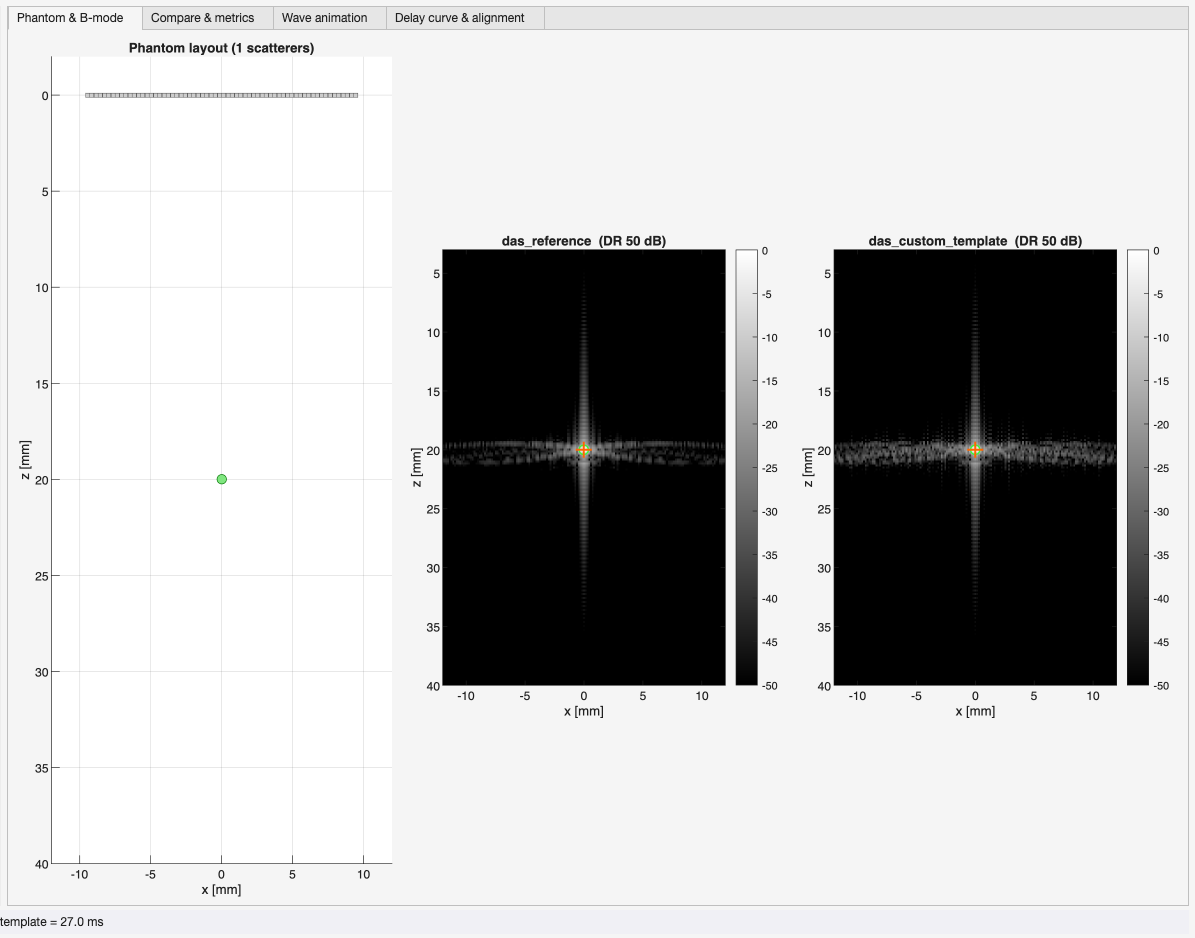
\includegraphics[width=0.92\textwidth]{figures/gui_bmode_crop.png}
  \caption{Phantom \& B-mode tab: a single point target reconstructed with
  the reference DAS (left) and a user-supplied algorithm (right), here the
  unmodified naive template, under identical acquisition settings.}
  \label{fig:gui-bmode}
\end{figure}

\begin{figure}[t]
  \centering
  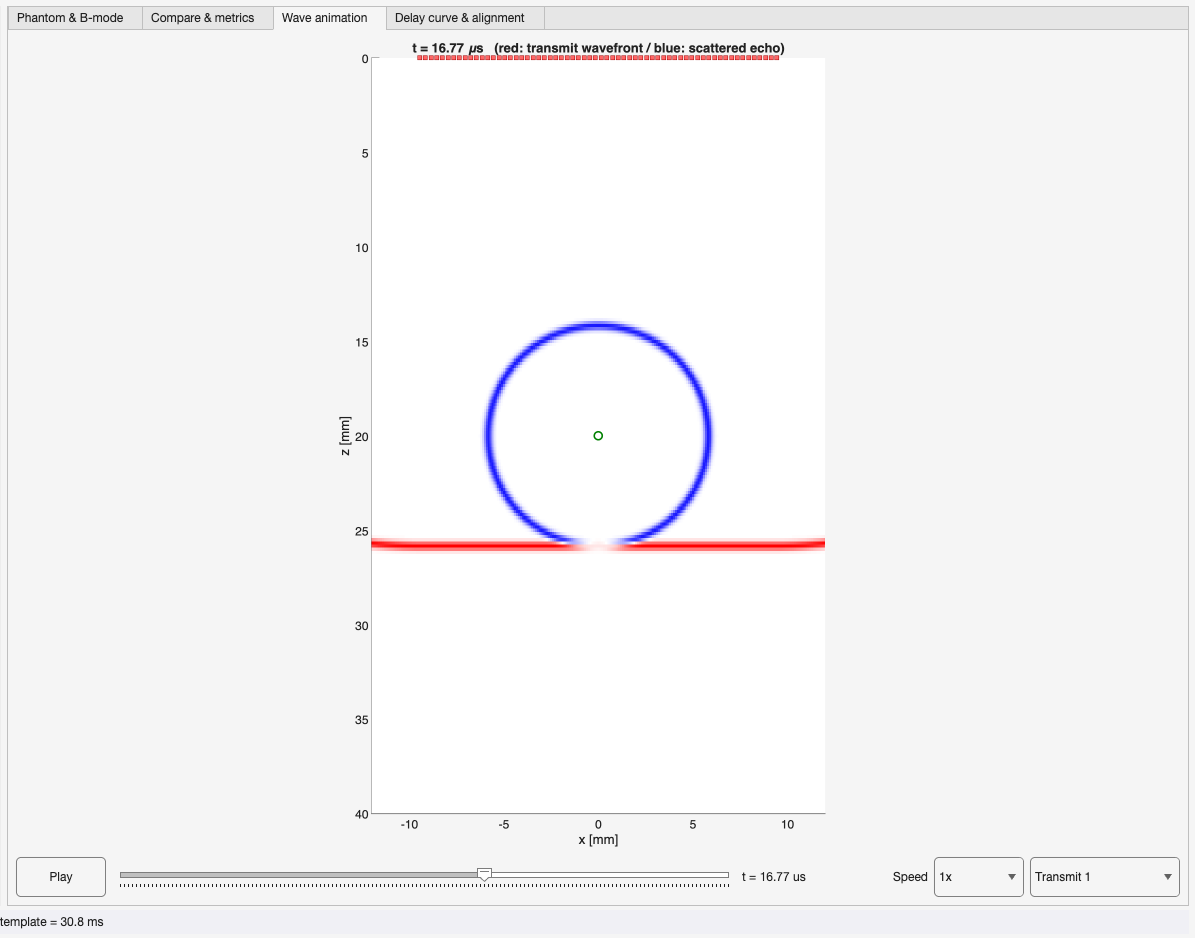
\includegraphics[width=0.6\textwidth]{figures/gui_anim_crop.png}
  \caption{Wave animation tab: the transmit wavefront (red, top) and the
  scattered echo (blue circle) expanding from the point target, drawn from
  the same transmit arrival-time model the beamformer uses.}
  \label{fig:gui-anim}
\end{figure}

\begin{figure}[t]
  \centering
  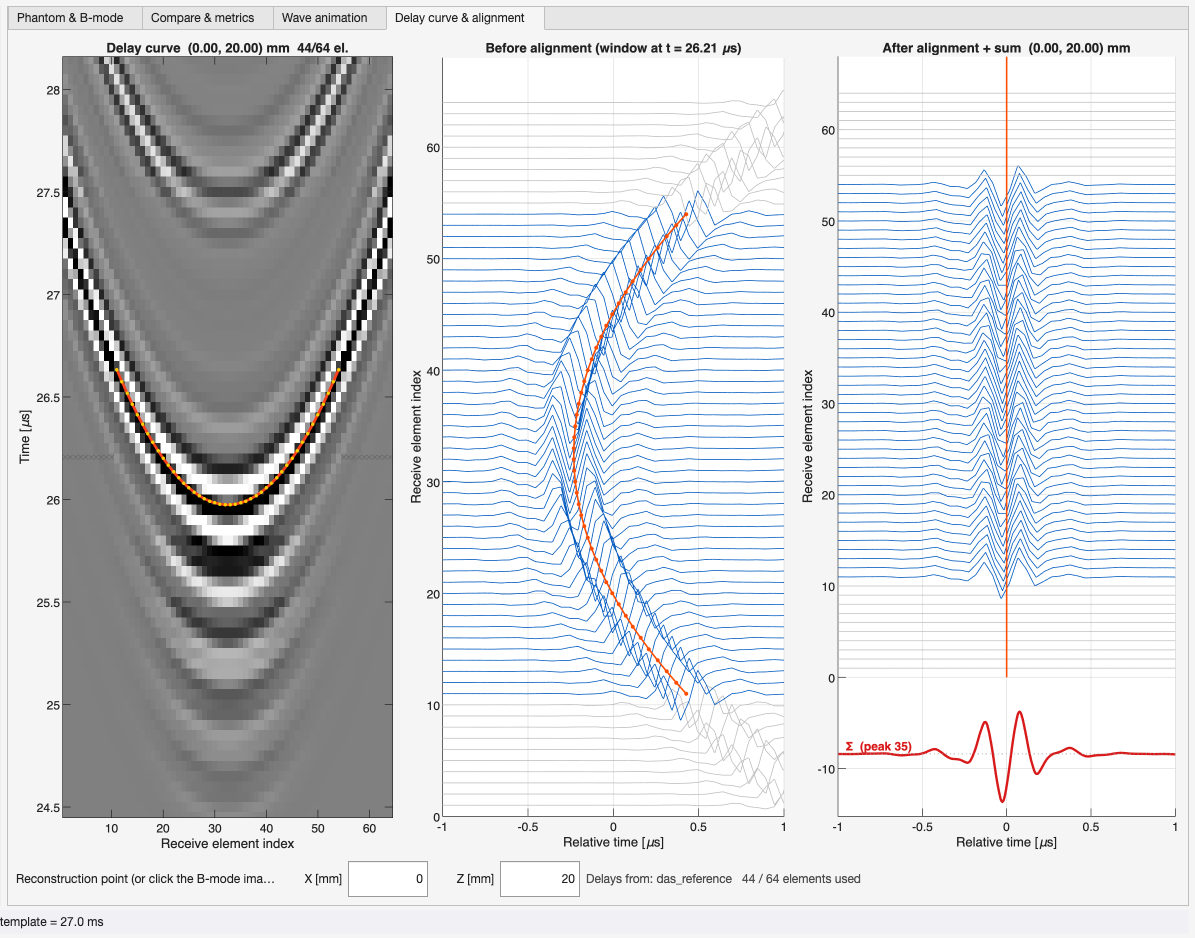
\includegraphics[width=0.98\textwidth]{figures/gui_delay_crop.png}
  \caption{Delay curve \& alignment tab, for the reconstruction point marked
  in Fig.~\ref{fig:gui-bmode}. Left: the RF data of every receive channel
  with the exact summed-sample locations overlaid as a curve. Middle: the
  same channels windowed around a common time, visibly out of phase. Right:
  the channels after delay correction, in phase, with their coherent sum
  drawn beneath.}
  \label{fig:gui-delay}
\end{figure}

\section{Two transmit-arrival-time models}
\label{sec:models}

The beamformer needs, for every reconstruction pixel $p$, the time at which
the transmitted wavefront reaches $p$. Two models are used, and using the
wrong one for a given transmit scheme is a plausible mistake for anyone
implementing this from scratch, which is why the tool exposes the choice
explicitly rather than hiding it inside a single opaque function.

\paragraph{First-arrival (Huygens) model.} For plane, diverging, and
single-element transmission,
\begin{equation}
  \tau_{\mathrm{tx}}(p) = \min_{e \in \mathrm{active}} \Big( d_e + \frac{|p - e|}{c} \Big),
  \label{eq:huygens}
\end{equation}
where $d_e$ is the programmed transmit delay of element $e$ and $c$ the
speed of sound. This is exact for these three schemes: it reduces to the
closed-form plane-wave expression $\tau = (x\sin\theta + z\cos\theta)/c$ and
to the equivalent diverging-wave expression under the corresponding delay
law, with no scheme-specific branching required.

\paragraph{Virtual-source model.} Applying Eq.~\eqref{eq:huygens} to a
focused transmit is exact \emph{before} the focus, but beyond it the
minimum is achieved by the aperture edge element's edge wave rather than by
the converged wavefront, which reconstructed images position roughly a
millimeter shallower than the true target depth in our tests. The tool
instead treats a focused transmit as a spherical wave passing through the
focal point $F$,
\begin{equation}
  \tau_{\mathrm{tx}}(p) = T_F + s \cdot \frac{|p - F|}{c}, \qquad
  s = \begin{cases} -1 & \text{before the focus} \\ +1 & \text{beyond it,} \end{cases}
  \label{eq:vsource}
\end{equation}
where $T_F$, the instant the wavefront converges on $F$, is recovered
directly from the programmed delays ($T_F = \mathrm{mean}_e(d_e + |e-F|/c)$)
and is therefore independent of how those delays happen to be normalized.
Both models are implemented identically in the reference beamformer and in
the wave animator, so the geometric object drawn in Fig.~\ref{fig:gui-anim}
is exactly what the beamformer in Fig.~\ref{fig:gui-delay} assumes.

\section{Analytic fallback RF model}
\label{sec:mock}

When \must{} is not installed, \code{sim\_engine.m} synthesizes RF data with
an analytic 2-D cylindrical-wave model: for every scatterer, the transmit
field at its location is built by superimposing the (delayed, obliquity- and
range-weighted) contributions of every active transmit element, and that
field is then propagated back to every receive element and accumulated into
the RF matrix, using the same speed of sound and delay laws the beamformer
uses. Element directivity, frequency-dependent attenuation, and rigorous
diffraction are not modelled; a Gaussian-modulated sinusoid, parameterized
by the probe's centre frequency and fractional bandwidth, stands in for the
pulse-echo waveform. The delay structure --- the geometric quantity a DAS
beamformer actually depends on --- is exact by construction, since it is
computed from the same closed-form and virtual-source expressions the
beamformer itself uses.

\section{Validation against \must}
\label{sec:validation}

\subsection{Method}

We compare the analytic fallback against \must's \textsc{simus} on seven
cases spanning all three transmit schemes, on- and off-axis targets, and
16/64/128-element probes (Table~\ref{tab:cases}), using a 64-element,
0.30\,mm-pitch, 5\,MHz probe with 75\% fractional bandwidth and $f_s = 4
f_c$ except where the element count is varied. Both backends receive
identical transmit delay laws and identical scatterer positions, so any
difference in the resulting RF or beamformed image is attributable to the
RF generation step and not to a beamforming inconsistency. For every case
we measure:

\begin{enumerate}[leftmargin=*]
  \item \textbf{Timing agreement.} Whether the simulated echo arrives at the
  geometrically expected two-way time, checked independently of any
  cross-backend comparison, by locating the envelope peak of the center
  receive channel for a plane-wave, on-axis target.
  \item \textbf{Per-channel raw-RF agreement.} The normalized cross-correlation
  between the two backends' RF data on every active channel, from which we
  report the mean peak correlation coefficient and, on the center channel,
  the sub-sample lag obtained by parabolic interpolation of the three
  \code{xcorr} samples around the integer-lag peak (\code{xcorr} itself only
  returns integer lags, so this step distinguishes a genuine near-integer
  offset from a quantized fractional one). The sign convention of the
  reported lag (which of the two backends a negative value means is
  earlier) is pinned down empirically, on a synthetic pair of signals with
  a hand-constructed known delay, by
  \code{validation/calibrate\_lag\_sign.m}, rather than assumed from
  \code{xcorr}'s documented convention.
  \item \textbf{Beamformed-image agreement.} Both RF data sets are
  beamformed with the identical reference implementation
  (\code{das\_reference.m}) on a common grid, and we report the Euclidean
  peak-position error against the known target and the lateral $-6$\,dB
  full width at half maximum (FWHM) of the linear envelope, located by
  sub-pixel linear interpolation of the half-maximum crossings.
\end{enumerate}

The lateral grid for the FWHM measurement uses 12.5\,\textmu m spacing
(1601 points over 20\,mm), substantially finer than the GUI's interactive
default (125\,\textmu m). This matters: at the coarser spacing, the focused
transmit's true mainlobe ($\approx 0.1$--$0.26$\,mm, see below) spans only
1--2 grid cells and its FWHM is dominated by grid quantization rather than
by the beam itself. We confirmed convergence by repeating the
focused-on-axis measurement at 125, 12.5, and 1.25\,\textmu m spacing; the
FWHM estimate changed by less than 0.1\% between the two finer grids,
confirming the coarsest grid was the outlier, not the other two.

All code for this comparison is in \code{validation/validate\_must\_vs\_mock.m}
in the repository, together with the raw output (CSV and figures) reported
here, so the comparison can be reproduced with \code{setup\_must} followed by
a single function call.

\begin{table}[t]
  \centering
  \caption{The seven validation cases. Target coordinates are (lateral,
  depth) relative to the array center; the focused case is on-axis with a
  20\,mm focal depth, the diverging cases use a 10\,mm virtual source
  depth.}
  \label{tab:cases}
  \begin{tabular}{lccc}
    \toprule
    Case & Scheme & Elements & Target (mm) \\
    \midrule
    plane\_onaxis      & plane      & 64  & (0, 20) \\
    plane\_offaxis     & plane      & 64  & (4, 25) \\
    focused\_onaxis    & focused    & 64  & (0, 20) \\
    diverging\_onaxis  & diverging  & 64  & (0, 20) \\
    diverging\_offaxis & diverging  & 64  & (4, 25) \\
    plane\_16el        & plane      & 16  & (0, 20) \\
    plane\_128el       & plane      & 128 & (0, 20) \\
    \bottomrule
  \end{tabular}
\end{table}

\subsection{Results}

\paragraph{Timing.} For a plane wave with an on-axis target at 20\,mm depth
($c=1540$\,m/s, expected two-way time $25.974\,\mu$s at the center element),
the mock backend's \emph{envelope} peak fell at $+0.51$ samples and \must's
at $-0.49$ samples relative to the geometric expectation, i.e.\ the mock's
envelope peak is about $1.00$ sample \emph{later} than \must's, and both are
within one sample of the geometric prediction. This confirms that $t_0 = 0$
(the convention both \code{sim\_engine} and the \must{} adapter use) is
correct for both backends, with no large systematic bias.

\paragraph{Raw-RF agreement.} Table~\ref{tab:results} reports, per case, the
mean per-channel peak correlation and the center-channel sub-sample lag,
obtained by cross-correlating the \emph{raw} (non-envelope) waveforms and
locating the peak with the sign convention verified empirically as
described above. The mean correlation across all
seven cases is $0.916$ (range $0.894$--$0.940$); it is lowest for the
128-element probe, the direction in which the mock's missing diffraction and
directivity terms would be expected to matter most. The raw-waveform
cross-correlation lag is consistently close to $-1.0$ samples ($-50$\,ns at
$f_s=20$\,MHz) across every scheme and element count (mean $-1.02$, range
$-1.08$ to $-0.94$), meaning the mock's raw waveform \emph{fine structure}
best aligns with \must's about one sample \emph{earlier} --- the opposite
sign from the envelope-peak comparison above, and this is expected rather
than contradictory: the two measurements probe different things. The
envelope-peak time tracks the pulse's group delay; the raw-waveform
cross-correlation lag tracks the alignment of its carrier oscillations
(phase). The two agree only when both signals are exact time-shifted copies
of one another. Figure~\ref{fig:rf-compare} (top) shows they are not: mock
uses a symmetric Gaussian-modulated sinusoid, \must{} a simulated
pulse-echo response with visibly different, less symmetric fine structure,
so a comparison keyed to the carrier phase (cross-correlation of the raw
waveform) and one keyed to the pulse envelope can disagree in sign while
both report a magnitude of about one sample. One sample is $50$\,ns, a
quarter of the $200$\,ns carrier period at 5\,MHz in either case --- well
below anything that would perceptibly shift a reconstructed image, and
consistent with a pulse-shape difference between the two backends rather
than with a delay-law disagreement.

\paragraph{Beamformed-image agreement.} Peak positions agree with the known
target and with each other to within about one lateral grid cell at the
finer grid ($\leq 0.14$\,mm; both backends use the same \code{tx\_info}
delay law for the beamformer's transmit-time model, so this is primarily a
grid/delay consistency check --- the small residual differences between the
two backends' peak positions, up to $\approx 0.09$\,mm, come from the
asymmetric \must{} pulse shifting the discrete argmax on a narrow mainlobe,
not from the delay law itself). Lateral FWHM agrees to within 10--20\% for
plane and diverging transmission (Table~\ref{tab:results},
Fig.~\ref{fig:summary} bottom). The exception is the on-axis focused case:
the mock's mainlobe is $0.10$\,mm wide against \must's $0.26$\,mm, a factor
of $2.6\times$, confirmed converged from 125\,\textmu m down to
1.25\,\textmu m grid spacing. We attribute this to the mock's missing
element directivity and finite-aperture diffraction, whose effect is
largest for the most tightly focused beam and comparatively minor for plane
and diverging transmission, where the beam is less concentrated to begin
with. As a rough independent check, the common rule-of-thumb approximation
for diffraction-limited lateral resolution, (f-number)$\times\lambda$, gives
$1.5 \times 0.308\,\mathrm{mm} \approx 0.46$\,mm for this probe and depth:
\must's $0.26$\,mm is already narrower than this order-of-magnitude estimate
(consistent with the coherent narrowing a two-way, dynamically-focused-on-
receive pulse-echo beam achieves relative to a simple one-way estimate),
while the mock's $0.10$\,mm is roughly $4$--$5\times$ narrower than the
rule-of-thumb value --- a mainlobe tighter than a simple diffraction
estimate would allow, independent of whether \must{} is taken as ground
truth. The 16-element case shows a different kind of discrepancy
($2.04$ vs.\ $1.61$\,mm mock vs.\ \must, mock \emph{wider} here rather than
narrower): with only 16 elements at 0.30\,mm pitch, the physical aperture is
4.5\,mm, well short of the 13.3\,mm the requested f/1.5 receive aperture
would want at 20\,mm depth, so the receive aperture is clipped to the full
array and the effective f-number is $\approx 4.4$, not $1.5$. This is a
distinct, aperture-limited regime rather than the same directivity effect
seen in the focused case (there, the 64-element, 18.9\,mm aperture is not
clipped), and we did not investigate the mock-vs-\must{} discrepancy in this
regime further.

\paragraph{Run time.} Excluding \must's approximately 20\,s one-time
per-session initialization cost (measured on the first \textsc{simus} call
of a fresh MATLAB session), steady-state per-call cost for both backends on
these small, single-scatterer scenes is a few milliseconds. This number is
sensitive to caching behaviour inside \must{} and is reported here only to
note that, once initialized, \must{} is not prohibitively slow for
interactive use of this size; it should not be read as a general
performance claim about either backend on larger, clinically realistic
scenes (e.g., the many-scatterer cyst phantom, which we did not run through
\must{} for this reason).

\begin{table}[t]
  \centering
  \caption{Validation results. Corr.\ is the mean per-channel peak
  cross-correlation between the mock and \must{} RF data. Sub-lag is the
  center-channel cross-correlation lag after parabolic sub-sample
  refinement (samples; $f_s=20$\,MHz for the 64/128-element cases,
  proportionally lower element count does not change $f_s$). FWHM is the
  $-6$\,dB lateral full width at half maximum of the beamformed linear
  envelope on a 12.5\,\textmu m grid.}
  \label{tab:results}
  \begin{tabular}{lccccc}
    \toprule
    Case & Corr. & Sub-lag & FWHM$_{\mathrm{mock}}$ (mm) & FWHM$_{\must}$ (mm) & Ratio \\
    \midrule
    plane\_onaxis      & 0.909 & $-1.03$ & 0.668 & 0.659 & 1.01 \\
    plane\_offaxis     & 0.910 & $-1.08$ & 0.755 & 0.738 & 1.02 \\
    focused\_onaxis    & 0.926 & $-1.00$ & 0.102 & 0.261 & 0.39 \\
    diverging\_onaxis  & 0.940 & $-0.94$ & 0.678 & 0.658 & 1.03 \\
    diverging\_offaxis & 0.918 & $-1.05$ & 0.590 & 0.708 & 0.83 \\
    plane\_16el        & 0.919 & $-1.04$ & 2.039 & 1.607 & 1.27 \\
    plane\_128el       & 0.894 & $-1.03$ & 0.668 & 0.659 & 1.01 \\
    \midrule
    Mean & 0.916 & $-1.02$ & 0.786 & 0.756 & --- \\
    \bottomrule
  \end{tabular}
\end{table}

\begin{figure}[t]
  \centering
  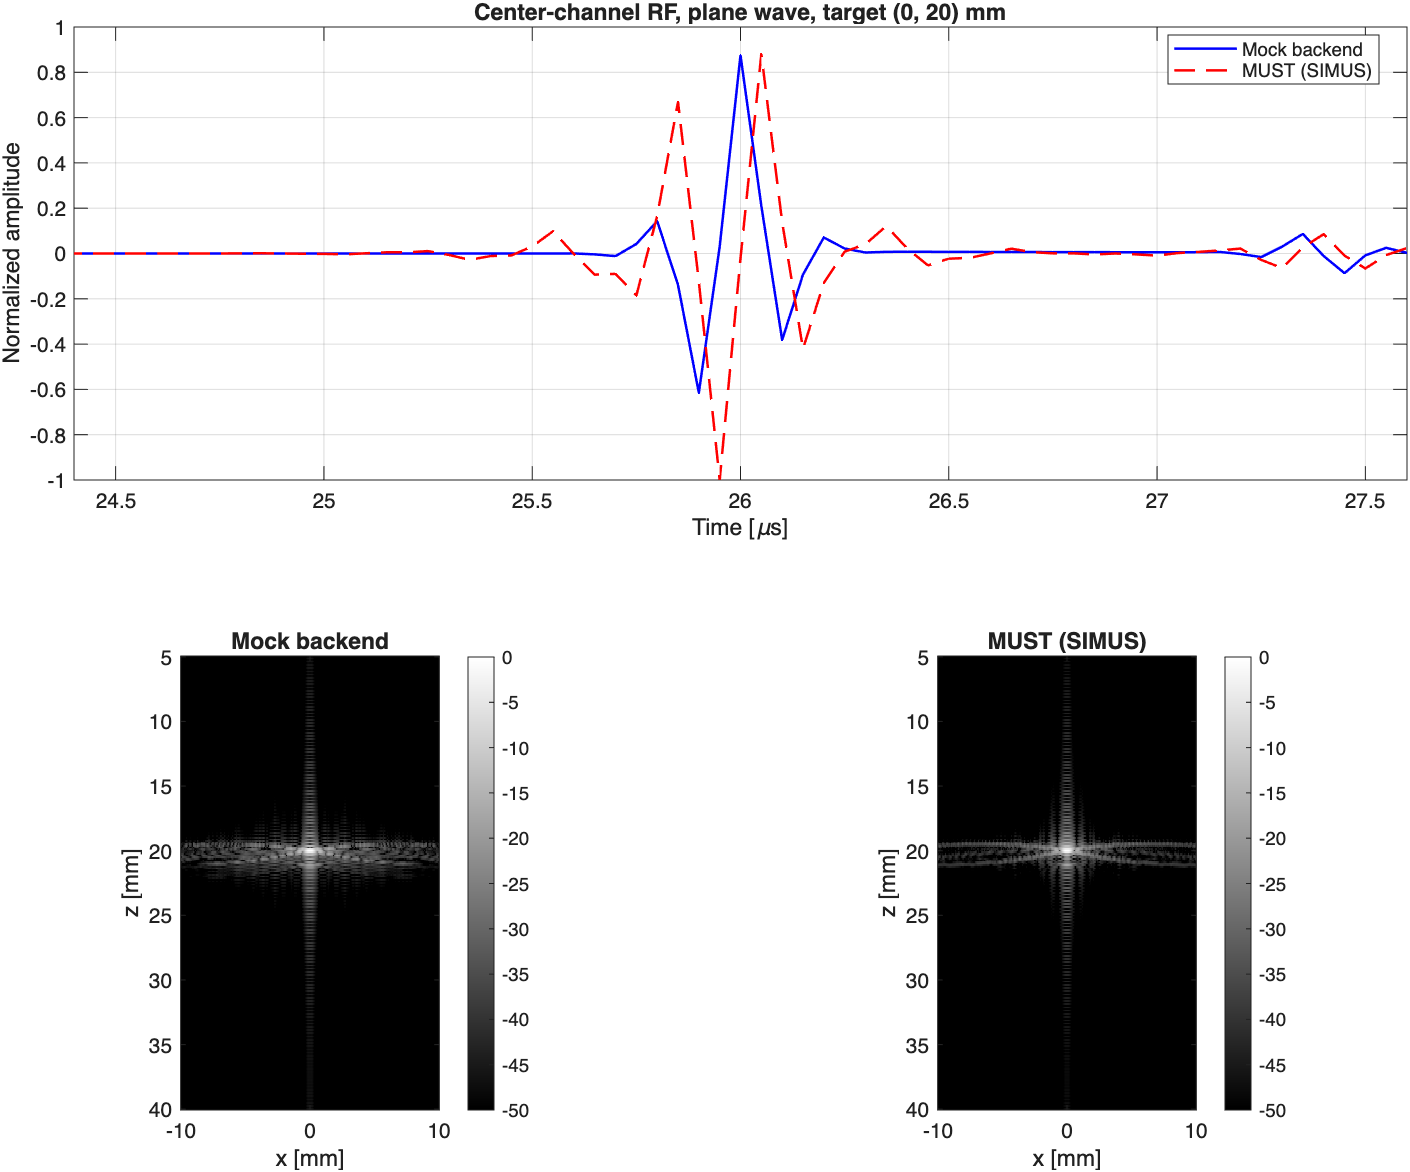
\includegraphics[width=0.95\textwidth]{figures/must_vs_mock_example.png}
  \caption{Top: center-channel RF trace for the on-axis plane-wave case,
  mock (blue) vs.\ \must{} (red dashed) -- same arrival time, visibly
  different pulse shape. Bottom: the corresponding beamformed B-mode images
  (50\,dB dynamic range), essentially indistinguishable for this scheme.}
  \label{fig:rf-compare}
\end{figure}

\begin{figure}[t]
  \centering
  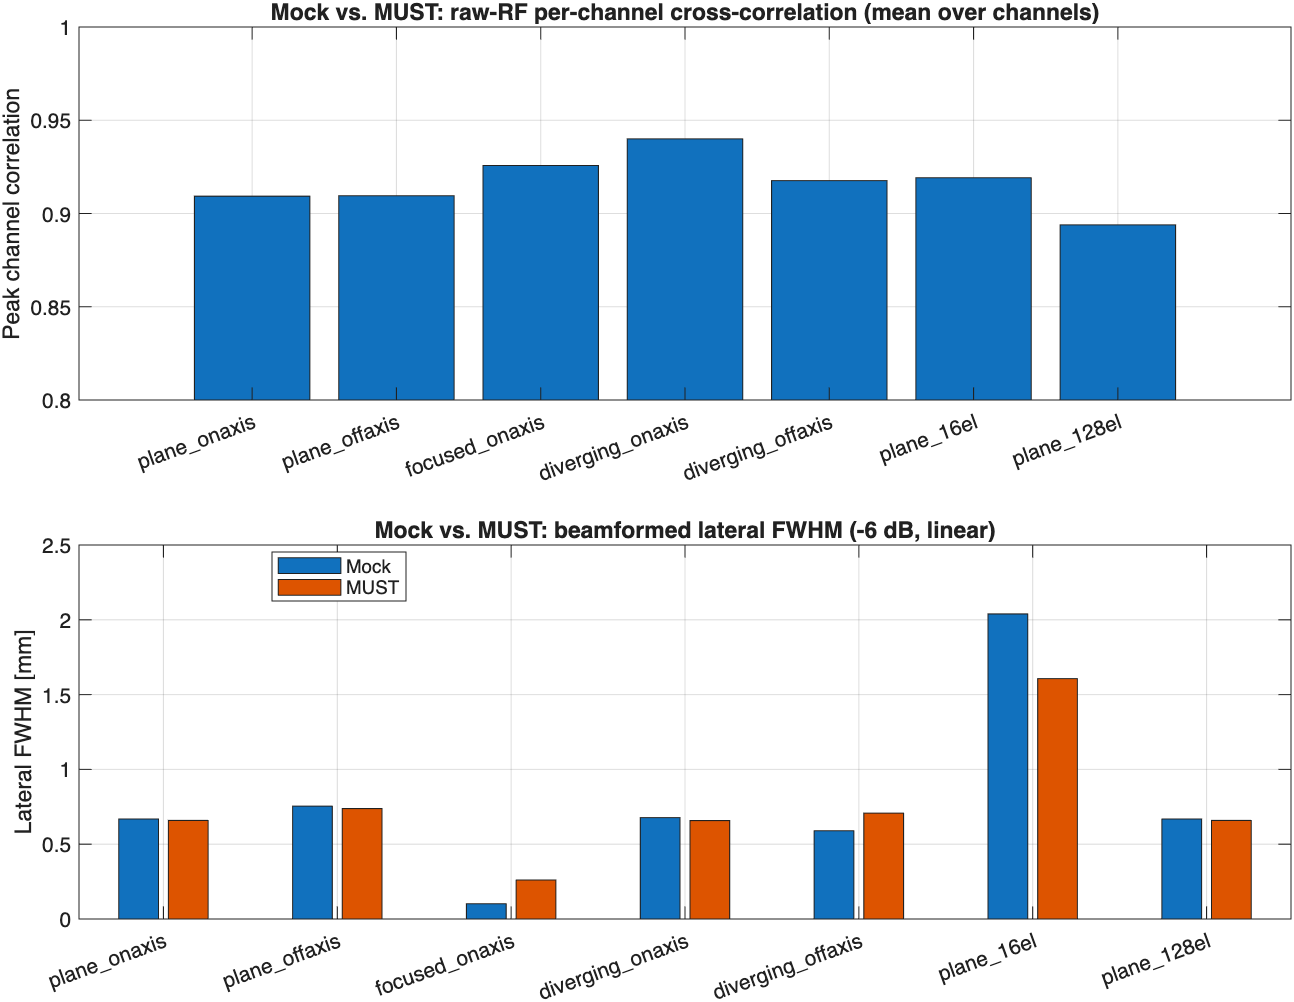
\includegraphics[width=0.85\textwidth]{figures/must_vs_mock_summary.png}
  \caption{Per-case summary. Top: raw-RF per-channel correlation. Bottom:
  lateral FWHM, mock vs.\ \must{}. The focused-on-axis case is the clear
  outlier, discussed in the text.}
  \label{fig:summary}
\end{figure}

\section{Limitations}
\label{sec:limitations}

\begin{itemize}[leftmargin=*]
  \item The simulation is 2-D only; elevation focusing, out-of-plane
  scattering, and 3-D array geometries are not modelled.
  \item The analytic fallback omits element directivity, finite-aperture
  diffraction, and frequency-dependent attenuation. Section~\ref{sec:validation}
  shows this is close to immaterial for plane and diverging transmission but
  causes the fallback to under-estimate focused-transmit lateral resolution
  by a factor of $\approx 2.6\times$; the fallback should not be used for
  quantitative image-quality or resolution claims about focused
  transmission, only for verifying beamformer delay logic.
  \item A focused transmit in this tool is a single scan line, not a
  laterally swept sequence; targets off the beam axis reconstruct as
  arc-shaped artefacts under either backend, by the physics of a single
  focused firing, not as a software defect.
  \item Multi-focus sequences are stitched by depth zone with independent
  envelope detection per zone, which introduces a faint seam (Hilbert
  transform edge effect) at each zone boundary.
  \item \must{} itself was only exercised on small, few-scatterer scenes for
  this validation (Section~\ref{sec:validation}); the reported per-call
  timing is not representative of large, clinically realistic scenes.
\end{itemize}

\section{Availability}

The source code, the validation scripts and results, and the \LaTeX{}
source of this manuscript are available at
\url{https://github.com/RyoMurakami-MedRobo/ultrasound-edu} under the MIT
license. \must{} itself is a separate dependency, licensed by its authors
under the GNU LGPLv3 and not bundled with this repository; a helper script
(\code{setup\_must.m}) downloads it from its official distribution point on
request.

\section{Conclusion}

We presented an open, dependency-light educational tool for exploring and
benchmarking delay-and-sum ultrasound beamforming, built so that a learner
can change the acquisition, see the transmit wavefront and the exact
samples a beamformer sums as explicit geometric objects, and drop in their
own algorithm under a single documented interface for quantitative
comparison against a reference implementation and against \must's built-in
beamformer. Because the tool's no-dependency fallback RF generator is the
only path guaranteed to run everywhere, we validated it quantitatively
against \must{} and found it timing-accurate and geometrically faithful,
with one clearly identified and quantified exception --- focused-transmit
lateral resolution --- that we report as a limitation rather than omit.

\bibliographystyle{unsrtnat}
\bibliography{refs}

\end{document}
